\documentclass{article}

\usepackage{amsmath, amssymb}
\usepackage[margin=0.8in]{geometry}
\usepackage{tikz}

\begin{document}

\section*{Example of Region of Interest}

\begin{figure*}
  \center
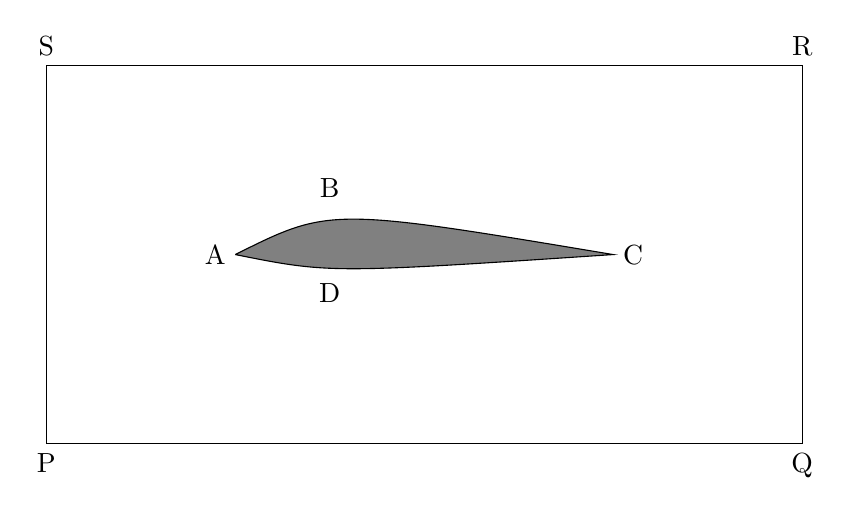
\begin{tikzpicture}[scale=1.2]
  \draw  (-4,-2) node[below] {P} -- (4,-2) node[below] {Q} -- (4,2) node[above] {R} -- (-4,2) node[above] {S} -- (-4,-2);
  \draw [fill=gray] (-2,0) node[left] {A} .. controls (-1,0.5) .. (2,0) node[right] {C} .. controls (-1,-0.2) .. (-2,0) ;
  \filldraw (-1,0.5) node[above] {B} ;
  \filldraw (-1,-0.2) node[below] {D} ;
\end{tikzpicture}

\caption{
As an example,
simulation of the airflow around an airfoil is modelled by a BVP.
Airfoils are objects of shapes which can,
for favourable airflow,
generate lift
(countering the gravitational forces)
like the wings of a turbine or aircraft.
For airflow simulation,
the Navier-Stokes Equations (NSE)
describe the physics
at each point in the domain
in the form of PDEs.
To specify the inflow, outflow
and the friction of the air with the airfoil
we impose boundary conditions
on the velocity and pressure
at the surface of the airfoil
and a rectangle around the airfoil
marking the region of interest (ROI).
\\
  The airfoil is shown with a grey colour,
  in the space between the curves ABC and ADC.
  The domain on which the Navier-Stokes Equations (NSE)
  are to be solved
  is the region between the outer rectangle PQRS
  and the airfoil.
  The boundary conditions on the velocity are pressure
  are imposed in the rectangle PQRS, curves ABC and ADC
  which form the boundary of the computational domain.
	}
\end{figure*}

\end{document}

